\section{Experimental Validation of SPNMF}
\label{sec:experiments}

In this section we conduct experiments to understand the behaviour of the proposed method. We first perform a test on a synthetic signal to validate the model of SPNMF in Section~\ref{SynthTest}. We then set-up the SPNMF to perform efficient source separation by quantifying the influence of the rank of factorization in Section~\ref{setup:rank}, the effect of different divergence in  Section~\ref{setup:divergence} and finally the performance of the separation with different types of dictionaries in  Section~\ref{setup:dictionary}.


\subsection{Synthetic Tests}\label{SynthTest}

To illustrate how the SPNMF with no dictionary works, we use a simple synthetic signal. The test signal models a mix of harmonic and percussive instruments. The harmonic part is simulated by a sum of sine waves that overlap in time and frequency. The first signal simulates a $C(3)$ with fundamental frequency $f_0 = 131$~Hz, the other one a $B(4)$ with $f_0 = 492$~Hz. To simulate the percussive part, for the first two seconds, we add $0.1$~s of Gaussian white noise. for the last two seconds, we add $0.3$~s of Gaussian white noise filtered by a high-pass filter. The signal is $5$~s long and the sampling rate is $4000$~Hz. We compute the Short Time Fourier Transform (STFT) with a $512$ sample-long ($0.128$~s) Hann analysis window and a $50\%$ overlap. The spectrogram of the signal is represented in Figure~\ref{SpectroSynth}. As our input signal has four sources, we expect that one source can be represented by one component and therefore, a model of rank 4 ($k=4$) should adequately model the signals. More precisely, for the NMF and the PNMF we chose $k=4$ and for the SPNMF $k'=2$ and $e=2$. The choice of the rank of factorization is an important variable of the problem, in this case, we select it in order to illustrate the performance of the method. We will further discuss the importance of the choice of the rank of factorization in Section~\ref{setup:rank}. We compare SPNMF with PNMF and NMF using the KL distance with multiplicative update rules as stated in~\cite{fevotte2009nonnegative}. The three algorithms are initialized with the same random positive matrices $W_{ini} \in \mathbb{R}^{n \times k}$  and $ H_{ini} \in \mathbb{R}^{k \times m}_{+} $.

The results of the decomposition are presented in Figure~\ref{resultONMF2}. The dictionary and activation matrix show the separation performance of the three methods. The NMF does not separate correctly the four components. By looking at the columns $2$ and $3$ of the dictionary matrix $W$ on Figure~\ref{resultONMF2}, the filtered Gaussian white noise and the $C(3)$ are separated in the same components which is not the expected result.
For the PNMF, the orthogonal components do not succeed to represent the two noises correctly. They are extracted in the same component and the total reconstruction error of the PNMF is high.
In this example, the SPNMF extracts the four components with the highest accuracy and performs better than the other methods. The two harmonic components are extracted in the orthogonal part (i.e., the columns $1$ and $2$ of the dictionary matrix) and the percussive components are extracted by the NMF part (columns $3$ and $4$). The SPNMF outperforms the two other methods and shows the potential of the algorithm for harmonic/percussive source separation.
%

\begin{figure}[htb]

  \centering 
  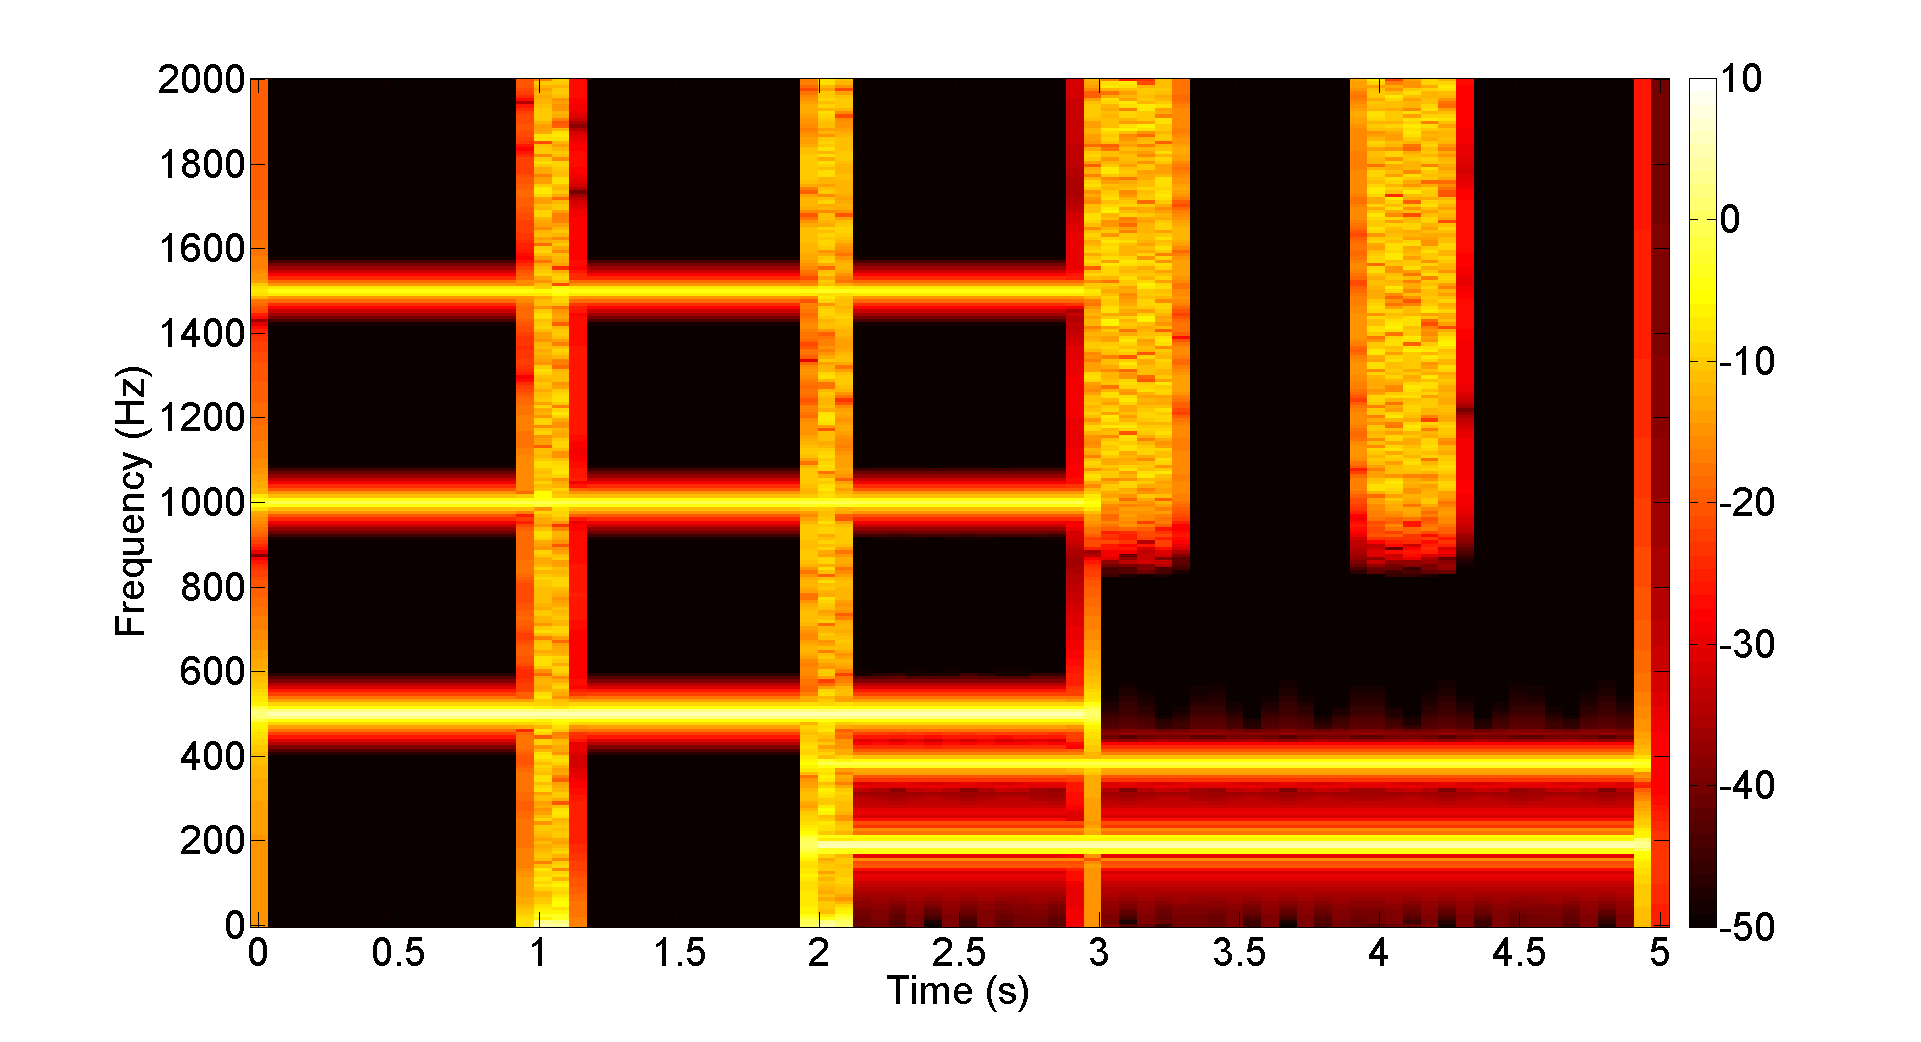
\includegraphics[width=9cm]{fig/synthetictestspectrogram.png}
%  \vspace{2.0cm}
  \caption{\label{SpectroSynth} Spectrogram of the synthetic test signals.}
  
\end{figure}

\begin{figure*}
   
	\centering    
  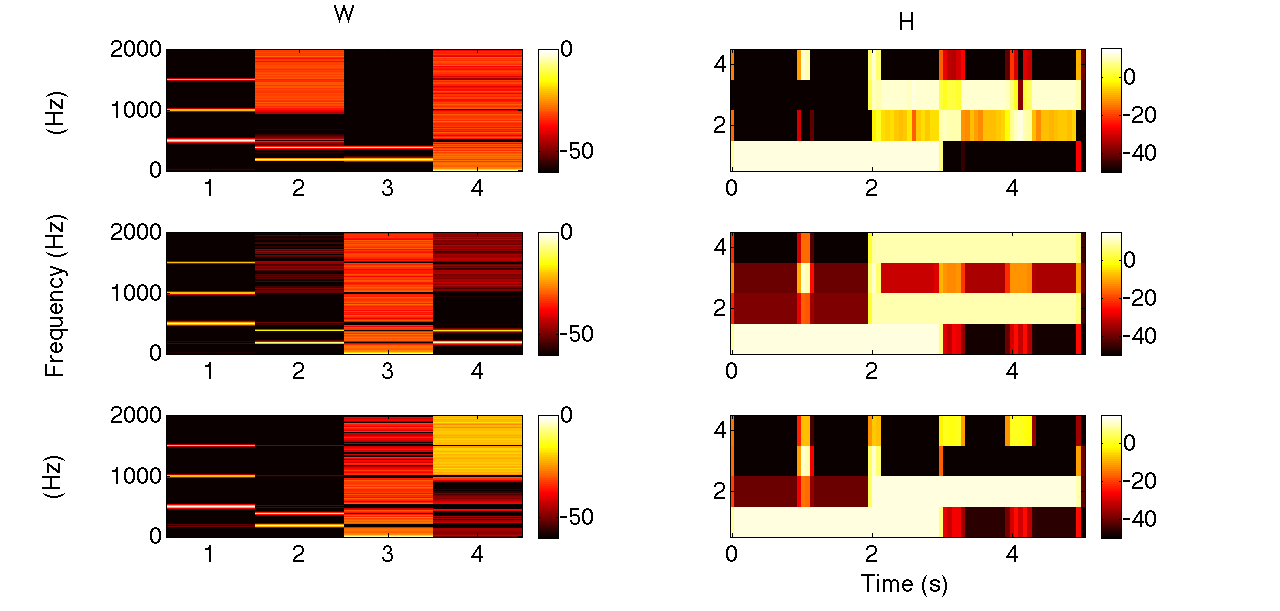
\includegraphics[width=15cm]{fig/WHcomp.png}

\caption{\label{resultONMF2} Results of the decomposition of the NMF (top matrices), PNMF (middle matrices) and SPNMF (bottom matrices).}


\end{figure*}


\subsection{Protocol and details of the test database}


To understand the behaviour of the SPNMF with the fixed dictionary (Algorithm~\ref{AlgoDictionary}), we run different tests on the public SiSec database from~\cite{SiSec10}. It is composed of polyphonic real-world music excerpts. Each music signal contains percussive, harmonic instruments and vocals. It consists of four recordings of duration ranging from $14$ to $24$~s. The goal is to perform an harmonic/percussive decomposition. Following~\cite{canadas2014percussive}, we will not consider the vocal part and we will build mixture signals only from the percussive and harmonic instruments. All the signals are sampled at $44.1kHz$. We compute the STFT with a $1024$ and $2048$ sample-long Hann window with a $50\%$ overlap.
Three tests are run on these data:
\begin{enumerate}
	\item The first test aims at assessing the robustness of the SPNMF with respect to the rank of the PNMF part. 
	\item The second test is to evaluate which of the three divergences (Euc, KL and IS respectively) give the best harmonic/percussive decomposition.
	\item The last test shows the influence of the dictionary on the separation performance. 
\end{enumerate} 
We are using a different database to set-up the proposed method from the one in the evaluation phase to prevent any possible over-training in order to make the comparison as fair as possible. 
In order to evaluate and compare the results we compute the common Signal to Distortion Ratio/Signal to Interference Ration/Signal to Artefact Ratio (SDR/SIR/SAR) metrics for blind source separation with the BSS-Eval toolbox~\cite{bsseval}. 


\subsection{Robustness wrt the rank of the harmonic part}
\label{setup:rank}

In the case where we use a dictionary matrix, the only parameter of the algorithm is the rank of factorization of the harmonic part. We used the SPNMF algorithm with the fixed dictionary obtained from the STFT of a drum signal as described in Section~\ref{fixedict}. The algorithms are implemented using the multiplicative update rules from~\ref{euclidisteq},~\ref{KLdisteq} and~\ref{ISdisteq} and they all are  initialized with the same random non-negative matrices. 
We display the mean value of the separation results on Figure~\ref{RankOfFact}. When the rank of factorization is small, the Euclidean distance and the KL divergence do not obtain satisfying results. However, for $r>=100$, the results for both distance are stable. With the IS divergence, the results seem independent of the size of the factorization.

The optimization process of SPNMF is straight forward thanks to the robustness of the method to the value of the rank of factorization. The number of components that can be decomposed by orthogonal basis functions are limited, and increasing the rank of factorization does not perturb the results as the harmonic part has to be orthogonal. For the rest of the article, the rank of factorization will be set to $r=100$ for all methods.



\begin{figure}[htb]

  \centering 
  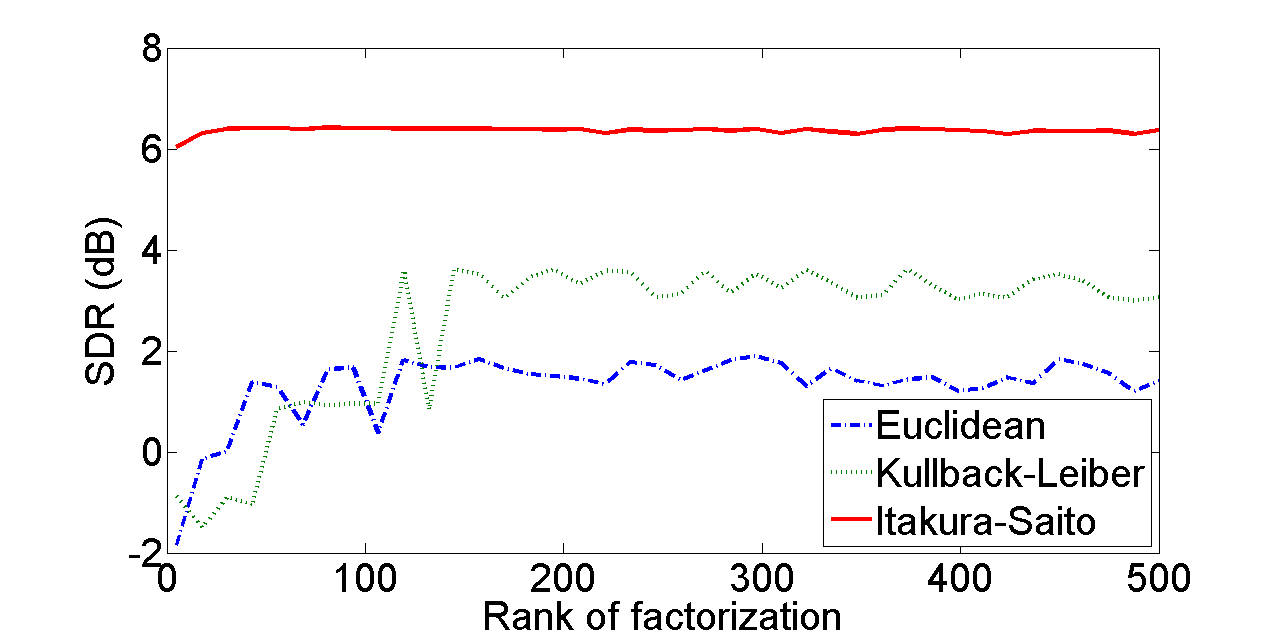
\includegraphics[width=9cm]{fig/RankOfFact.png}
%  \vspace{2.0cm}
  \caption{\label{RankOfFact} Optimization of the rank of factorization with the three divergences.}
  
\end{figure}




\subsection{Influence of the divergence}
\label{setup:divergence}

In this section we discuss the influence of the divergence in the results of the SPNMF algorithm. It has been established that the IS divergence is well suited to audio signal decomposition~\cite{gray1980distortion}, even if it does not always lead to superior separation performance~\cite{canadas2014percussive}. In this section, we perform a test of the three divergences on the SiSec database to evaluate the performance of the three algorithms. We tried two different windows length ($1024$ samples and $2048$ samples) for the Fourier transform as it showed interesting results. We display on Figures~\ref{frame1024} and~\ref{frame2048} the mean of the results of the three algorithms on the SiSec database. Each box-plot is made up of a central line indicating the median of the data, upper and lower box edges indicating the $1^{st}$ and $3^{rd}$ quartiles, and whiskers indicating the minimum and maximum values. 

When the frame length is small, the percussive instruments are well represented and the energy is localized. Using a longer window spreads the percussive energy while the tonal components are well separated in the TF domain.

When the frame size is small, Figure~\ref{frame1024} shows that the percussive decomposition is better for the Euclidean distance and the KL divergences, however, the harmonic components are not well separated in the TF domain, the orthogonal part of SPNMF does not perform a good separation.  
In the case of a long window, the Figure~\ref{frame2048} shows that the IS divergence performs better than the other divergences. The orthogonal part is more effective to extract the harmonic components as the finer frequency resolution allows for a better separation in the TF domain. The scale invariant property of the IS divergence meaning that low energy components of the spectrogram bear the same relative importance as high energy ones, allows a good extraction of the percussive instruments even if the energy is spread temporally.


For the rest of the article, we will use the SPNMF algorithm with the IS divergence and a $2048$ window size in the STFT.


\begin{figure}[htb]

  \centering 
  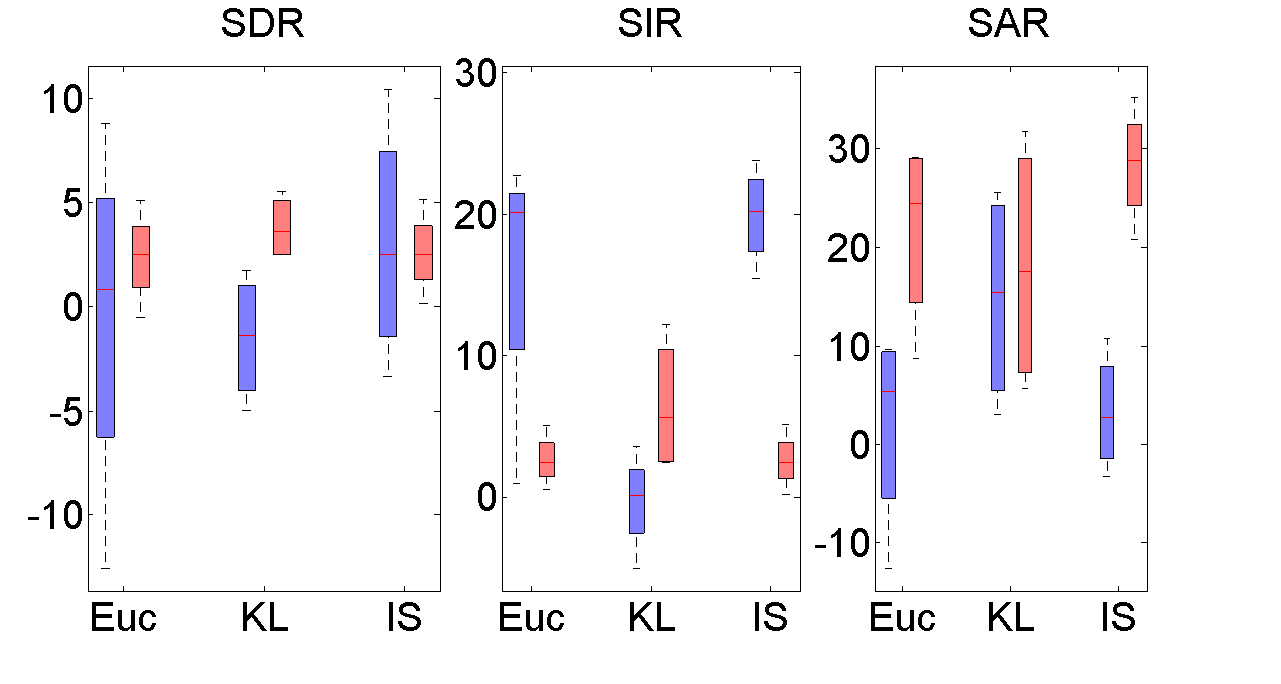
\includegraphics[width=9cm]{fig/DivergenceFrame1024.png}
%  \vspace{2.0cm}
  \caption{\label{frame1024} SDR, SIR and SAR of harmonic (left bar)/percussive (right bar) estimated sources on the SiSec database with a window frame of $1024$ samples.}
  
\end{figure}


\begin{figure}[htb]

  \centering 
  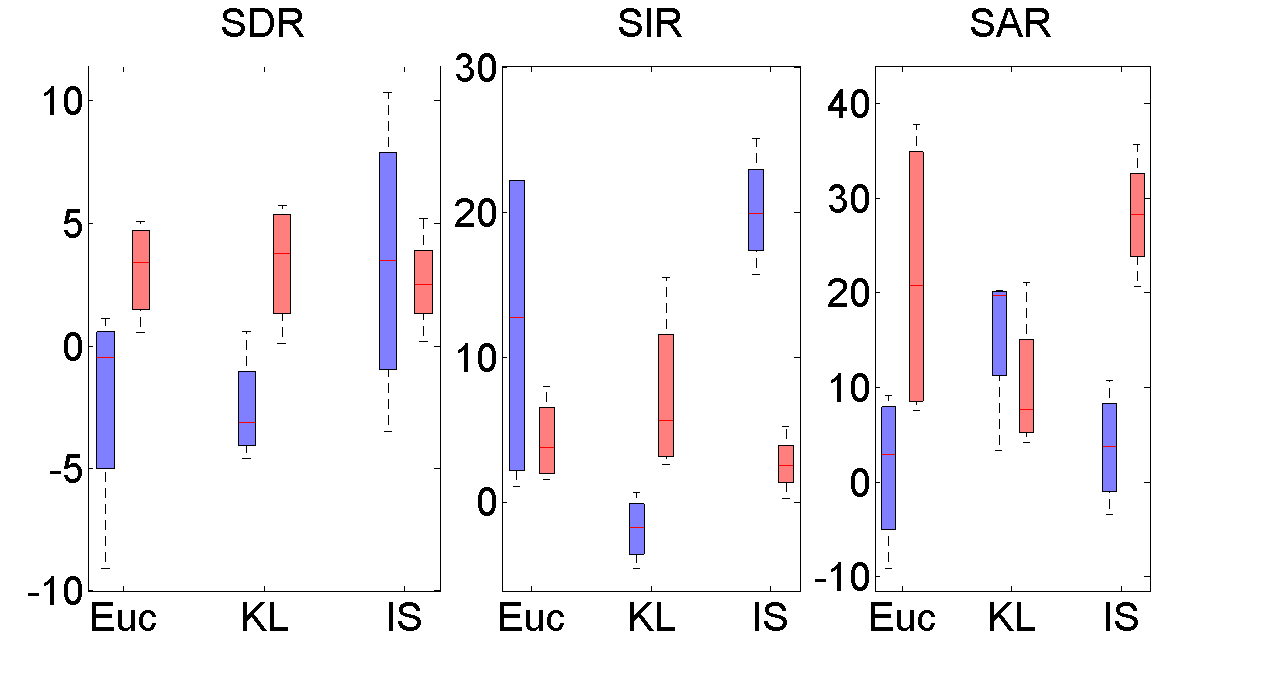
\includegraphics[width=9cm]{fig/DivergenceFrame2048.png}
%  \vspace{2.0cm}
  \caption{\label{frame2048} SDR, SIR and SAR of harmonic (left bar)/percussive (right bar) estimated sources on the SiSec database with a window frame of $2048$ samples.}
  
\end{figure}



\subsection{Influence of the dictionary}
\label{setup:dictionary}

We now discuss the influence of the dictionary. We tried the two methods described in Section~\ref{fixedict} and a third dictionary is made by the concatenation of the two dictionaries. The more information contained is the dictionary, the more chance for the decomposition to properly extract the percussive part. On some signals, the decomposition is not able to extract a lot of energy from the mixture as no atoms from the dictionary correspond to an atom of the percussive signal.
We display on Figure~\ref{resultsDict} the SDR results of the decomposition using the NMF dictionary, the STFT dictionary and the concatenated dictionary. The SAR and SIR are postponed in Appendix~\ref{appendix:dict} on Figures~\ref{resultsDictSAR} and~\ref{resultsDictSIR} respectively. On our tests, the results with the concatenated dictionary have the highest score. Indeed, the concatenated dictionary contains the largest amount of information and as a result, obtains the best separation. As the dictionary is fixed, it is important to have a large dictionary to extract a large type of percussive instruments. The STFT dictionary and the NMF dictionary obtain similar results. Each dictionary contain complementary information that allow for a better separation well they are concatenated. For the tests we will conduct later in Section~\ref{sec:stateoftheart} on a large database, we will use the concatenated dictionary as it contains the largest amount of information. 


\begin{figure}[htb]

  \centering 
  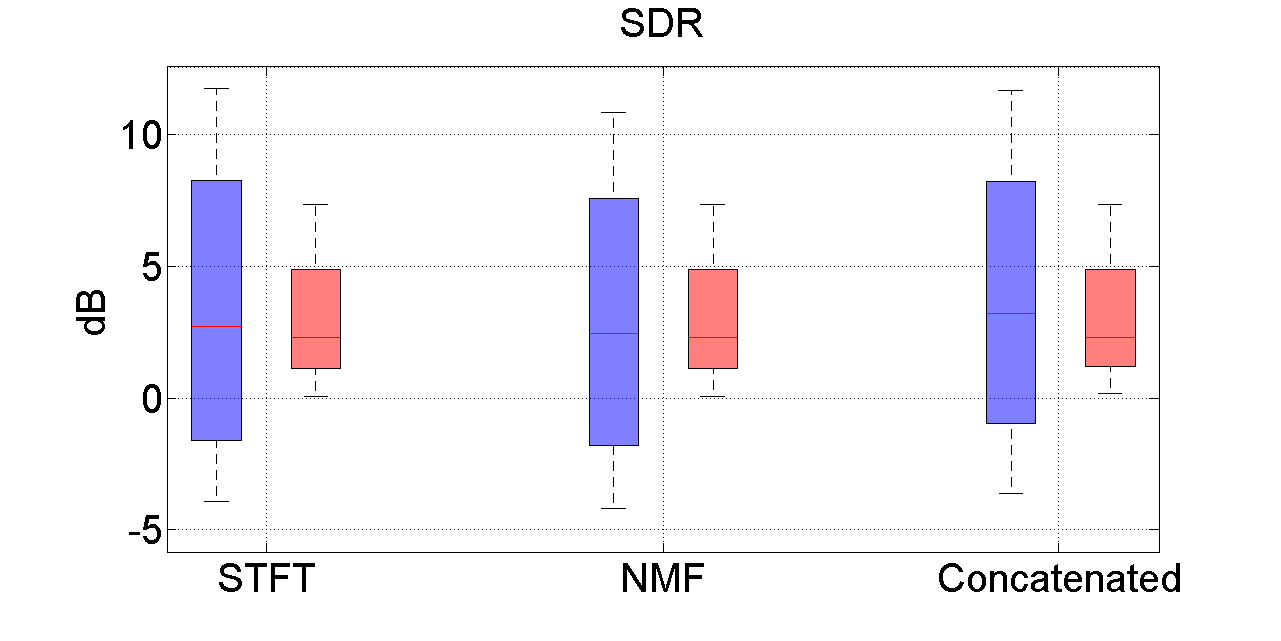
\includegraphics[width=8cm]{fig/DictSDR.png}
%  \vspace{2.0cm}
  \caption{\label{resultsDict} SDR of harmonic (left bar)/percussive (right bar) estimated sources on the SiSec database with a STFT dictionary, a NMF dictionary and the concatenation of the two.}
  
\end{figure}


%\begin{table}
%   
%	\centering    
%   \begin{tabular}{|l|l|l|l|l|}
%  \hline
%  &    & Percussive separation & Harmonic separation  \\
%  \hline
%       & NMF          & 10.28 & 2.69  \\
%  SDR  & STFT         & 10.17 & 2.59  \\
%  (dB) & Concatenated & 10.21 & 2.51  \\  
%  \hline
%       & NMF           & 20.97 & 2.45  \\
%  SIR  & STFT          & 21.11 & 2.61  \\
%  (dB) & Concatenated  & 20.70 & 2.65  \\  
%   \hline
%       & NMF           & 10.70 & 29.41  \\
%  SAR  & STFT          & 10.58 & 29.59  \\
%  (dB) & Concatenated  & 10.65 & 29.58  \\ 
%  \hline
%\end{tabular} 
%\caption{\label{resultsDict} Source separation performance using three dictionaries.}
%
%
%\end{table}
%\vspace{-0.4cm}
%
